\chapter*{\textbf{Эксперимент №6: Сравнение алгоритмов сортировки}}
\addcontentsline{toc}{chapter}{Эксперимент №6: Сравнение алгоритмов сортировки}

\subsection*{\textbf{Цель эксперимента}}
Исследование способов эффективного использования памяти и выявление наиболее эффективных алгоритмов сортировки, применимых в вычислительных системах. 

\subsection*{\textbf{Исходные данные}}
Количество процессоров вычислительной системы, размер пакета, количество элементов в массиве, разрядность элементов массива.

\subsection*{\textbf{Описание проблемы}}
Существует несколько десятков алгоритмов сортировки. Их можно классифицировать по таким критериям, как: назначение (внутренняя и внешняя сортировки), вычислительная сложность (алгоритмы с вычислительными сложностями $O(n^2), O(n*log(n)), O(n), O(n/log(n))$), емкостная сложность (алгоритмы, требующие и не требующие дополнительного массива), возможность распараллеливания (нераспараллеливаемые, ограниченно распараллеливаемые, полностью распараллеливаемые), принцип определения порядка (алгоритмы, использующие парные сравнения и не использующие парные сравнения).  

\subsubsection{\textbf{Radix Sort}}

Логика данной сортировки проста. Допустим, у нас есть массив из 10 чисел.

Сначала идет сортировка их по первому (старшему) разряду. Сортировка в таком случае выполняется с помощью сортировки подсчетом (count sort). Сложность — $O(n)$. 

В итоге получается 10 «корзин» — в которых старший разряд 0, 1, 2 и т.д.

Далее в каждой из корзин запускаем ту же процедуру, но только рассматриваем уже не старший разряд, а следующий за ним, и т.д.

Такие действия выполняется до последнего разряда.

\subsection*{\textbf{Результаты эксперимента}}
На рисунке \ref{img:experiment_6} предаставлен график, полученный в результате эксперимента с исходными параметрами:
\begin{itemize}
	\item Количество 64-х разрядных элементов массивов (М) = 1;
	\item Шаг увеличения размера массива (К) = 32.
\end{itemize}

\begin{figure}[H]
	\centering{
		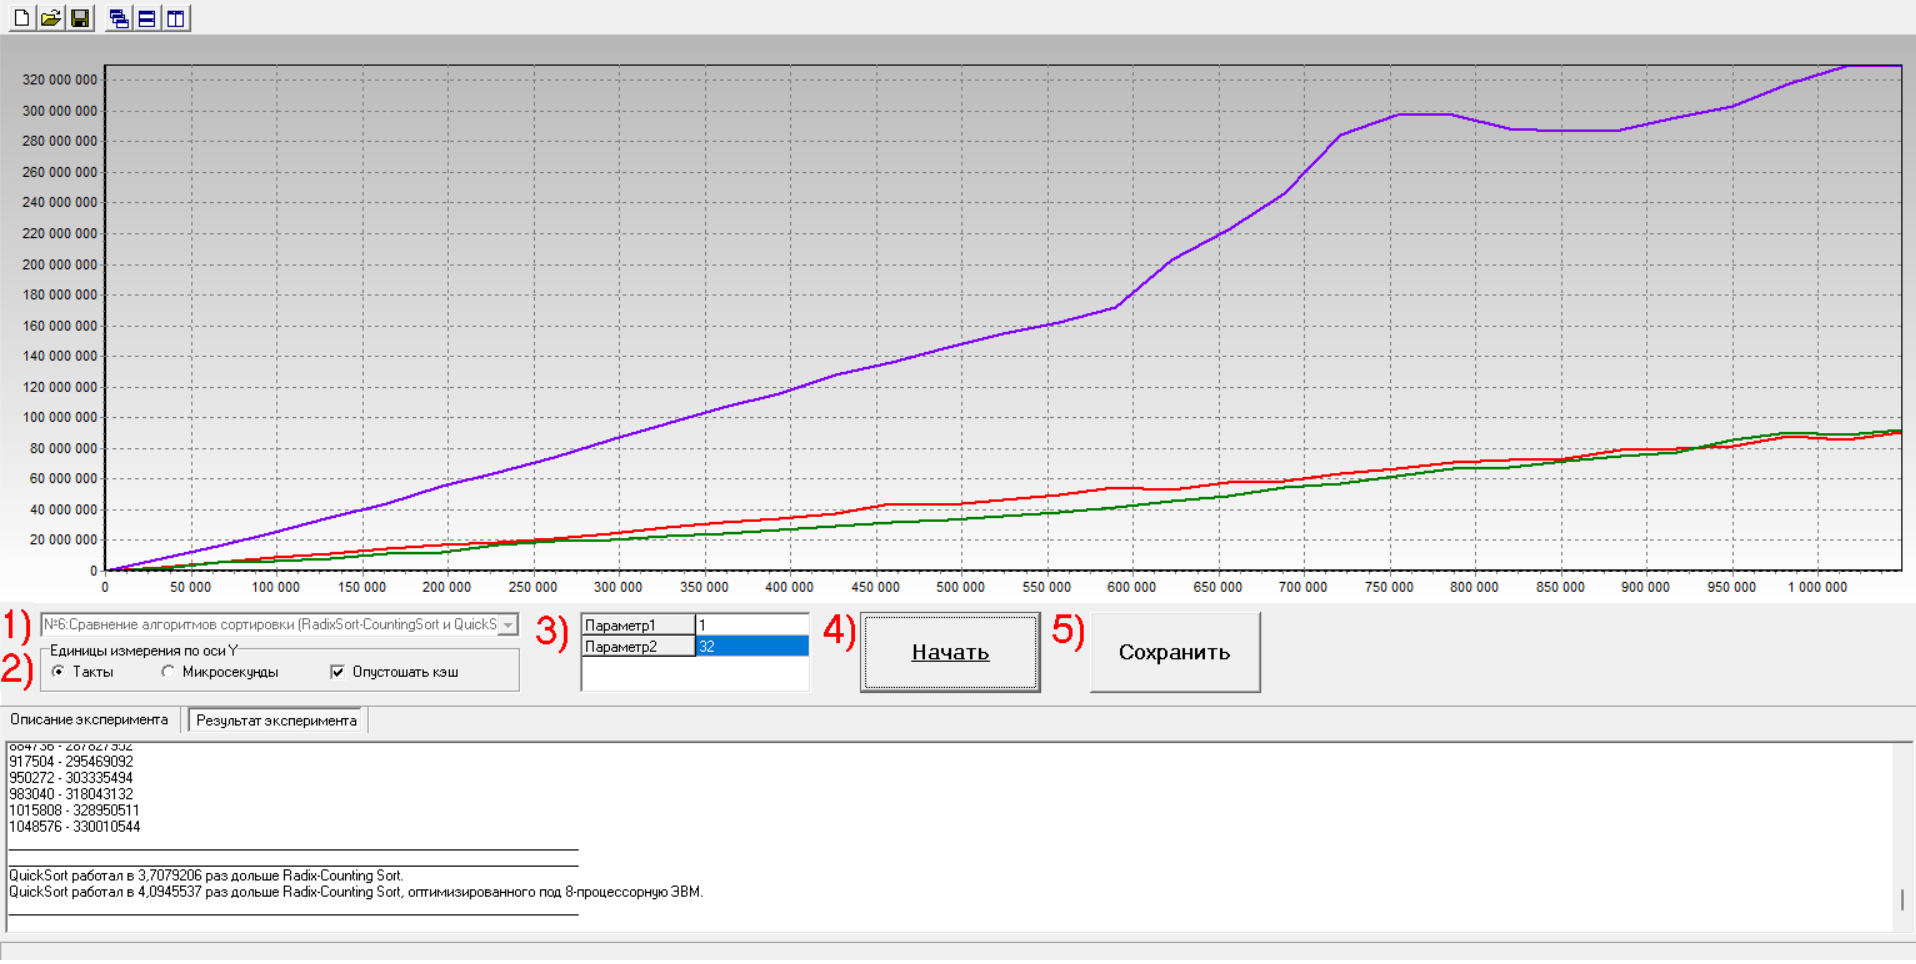
\includegraphics[scale=0.4]{images/experiment_6_1}
		\caption{Эксперимент №6}
		\label{img:experiment_6}
	}
\end{figure}

Результат сравнения времени (как вывод программы) представлен на рисунке \ref{img:experiment_6}. Как видно на рисунке, QuickSort работал в 3,7079206 раз дольше Radix-Counting Sort, и QuickSort работал в 4,0945537 раз дольше Radix-Counting Sort, оптимизированного под 8-процессорную ЭВМ.

Фиолетовый график показывает время или количество тактов работы алгоритма QuickSort. 

Красный график показывает время или количество тактов работы неоптимизированного алгоритма Radix-Counting. 

Зеленый график показывает время или количество тактов работы оптимизированного под 8-процессорную вычислительную систему алгоритма Radix-Counting.

\subsection*{Вывод}
Существует сортировка, работающая быстрее чем QuickSort, при этом, даже ее можно еще оптимизировать для более быстрой работы.